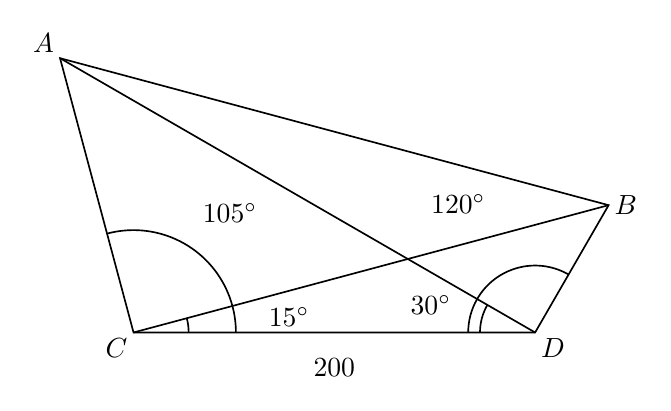
\begin{tikzpicture}[x=1cm,y=1cm,font=\normalsize,
 geometry edge/.style={solid,line width=.6pt},
 geometry mark/.style={solid,line width=.6pt},
 geometry label/.style={font=\normalsize,inner sep=2pt}]
\coordinate (A) at (0.341700000,3.483300000);
\coordinate (B) at (7.308300000,1.616700000);
\coordinate (C) at (1.275000000,0.000000000);
\coordinate (D) at (6.375000000,0.000000000);
\coordinate (T105) at (2.500000000,1.520000000);
\coordinate (T15) at (3.250000000,0.200000000);
\coordinate (T30) at (5.050000000,0.350000000);
\coordinate (T120) at (5.400000000,1.630000000);
\coordinate (T200) at (3.825000000,-0.450000000);
\draw[geometry edge] (A)--(B)--(D)--(C)--cycle;
\draw[geometry edge] (A)--(D);
\draw[geometry edge] (B)--(C);
\draw[geometry mark] (C) ++(0:1.3) arc (0:105:1.3);
\draw[geometry mark] (C) ++(0:0.7) arc (0:15:0.7);
\draw[geometry mark] (D) ++(150:0.7) arc (150:180:0.7);
\draw[geometry mark] (D) ++(60:0.85) arc (60:180:0.85);
\node[geometry label,above left] at (A) {$A$};
\node[geometry label,right] at (B) {$B$};
\node[geometry label,below left] at (C) {$C$};
\node[geometry label,below right] at (D) {$D$};
\node[geometry label] at (T105) {$105^\circ$};
\node[geometry label] at (T15) {$15^\circ$};
\node[geometry label] at (T30) {$30^\circ$};
\node[geometry label] at (T120) {$120^\circ$};
\node[geometry label] at (T200) {$200$};
\end{tikzpicture}
